 % Source: http://tex.stackexchange.com/a/150903/23931
\documentclass[11pt]{article}
\renewcommand{\baselinestretch}{1.05} 
% \usepackage[letterpaper,margin=.95in,top=0.8in,tmargin=1in]{geometry}
\usepackage[letterpaper,margin=.70in]{geometry}
\usepackage{xcolor}
\usepackage{fancyhdr}
\usepackage{tgschola} % or any other font package you like
\usepackage{mathptmx}
\usepackage{graphicx}
\usepackage{soul}
\usepackage[font=scriptsize]{caption}
\usepackage[
	sorting=none,
	backend=bibtex,
	style=phys,
	maxcitenames=1,
	maxbibnames=2,
	natbib=true,
	giveninits=true]{biblatex}
\addbibresource{main.bib}
\usepackage{multicol}
\usepackage{setspace}
\renewcommand*{\bibfont}{\scriptsize}	

% \pagestyle{fancy}
% \fancyhf{}
% \lhead{\large Personal Statement\\
% \small October 31, 2025}
% % \chead{\large \textsc{ School Name }\\
% % \small{Department of Physics}}
% \rhead{\large Prakruth Adari\\
% \small{Postdoc Applicant}}
% \rfoot{\thepage}


\newcommand{\yourname}{Prakruth Adari}


\definecolor{linkcolor}{rgb}{0,0,1}
\usepackage[
  colorlinks,
  breaklinks,
  urlcolor=linkcolor,
  linkcolor=linkcolor,
  citecolor=linkcolor,
  pdftitle={\yourname},
  pdfauthor={\yourname},
  unicode
]{hyperref}


\newcommand{\PersonalTag}[4][black]{{\color{#3}{$^{#2}$[}}{\color{#1}#4}{\color{#3}]}}
\definecolor{darkpastelpurple}{rgb}{0.59, 0.44, 0.84}
\newcommand{\pa}[2][darkpastelpurple]{\PersonalTag[#1]{Prakruth}{darkpastelpurple}{#2}}


\begin{document}

\pagestyle{fancy}
\fancyhead[L]{Research Statement}
\fancyhead[R]{Prakruth Adari}

\indent \indent The fundamental nature of dark energy and dark matter are some of the most exciting questions in physics pushing the limits of our understanding of the cosmos.
I am interested in using galaxy clusters to probe these mysteries specifically focusing on the evolution of cosmological parameters like $\sigma_8$ and $\Omega_M$ through cluster weak lensing.
With the Vera Rubin Observatory beginning its 10 year survey of the southern sky, Euclid's first data release in October 2026, and Roman's successful launch, this is an extremely exciting time for all of astronomy including cluster weak lensing.
While exciting, there are a number of systematics that need to be dealt with to make the most of the data especially as we push to smaller non-linear scales.
During my PhD I have focused on one systematic, blending, along with making some of the first weak lensing measurements with the Vera Rubin Observatory by studying a galaxy cluster Abell 360.
I propose to continue working on both weak lensing systematics and cluster science measurements during my postdoc specifically focusing building and validating tools that can enable high quality tomographic measurements.



% I am extremely excited by the prospects of probing both of these mysteries through galaxy cluster weak lensing with the Vera Rubin Observatory and Roman space telescope.
% Specifically, I am interested in the evolution of cosmological parameters like $\sigma_8$ and $\Omega_M$ which can give robust tests of general relativity and dark energy.
% Galaxy clusters are some of the largest gravitationally bound objects offering a rich laboratory to conduct these studies whether through cluster count cosmology or gas fraction studies.
% % jWith the latest DESI results preferring an evolving dark energy, a late and early universe tensions like $H_0$, I am very interested in studying cosmology through multiple redshifts which clusters are 
% % jGalaxy clusters are rich laboratories to probe the universe probing cosmology through the halo mass function, dark matter constraints through density profiles, and gravity through the growth of structure.
% % jThe overwhelming amount of data coming from these telescopes will not only enable these studies but also allow for testing on redshift dependnce of parameters which I find very interesting.
% % \pa{Make this transition nicer} Galaxy clusters are great! We can get cosmology through the halo mass function, dark matter constraints through density profiles, and even constraint baryonic feedback through the gas fraction of clusters.
% While promising, there are a number of systematics that need to be dealt with to make the most of the data especially as we push to smaller non-linear scales.
% During my phd I have focused on one systematic, blending, along with making some of the first weak lensing measurements with the Vera Rubin Observatory by studying a galaxy cluster. 
% I propose to continue working on both weak lensing systematics and cluster science measurements during my postdoc specifically focusing on the systematics and measurements at small scales.


\indent \indent Blending generically refers to any instance when flux along a line of sight can be attributed to multiple objects and I have focused on an extreme case, unrecognized blends, in which two galaxies are mistakenly detected as a single object (example shown in Fig~\ref{fig:blend_ex}).
Unrecognized blends can bias basic photometry and shape measurements which will impact the capability to produce precision weak lensing results.
Moreover, it is expected that 20\% to 30\% of LSST-detected objects will be unrecognized blends making this an unavoidable and somewhat unmitigated problem \cite{roman_rubin}.
The repercussions of unrecognized blends via detection bias alone have been studied previously, showing shifts in cosmology parameters at the level of a few percent \cite{ben_clustering, blends_2011, kidsblends_2025}, and an early study including the impact on shape and flux measurements found up to a 2$\sigma$ shift in S$_8$ when conducing a cosmic shear analysis \cite{erfan}.
Mitigating the effects of these objects on weak lensing measurements is not straightforward as they couple both redshift and shears requiring a joint strategy.
The process of producing a joint redshift-shear calibration for these effects is outlined in \cite{maccrann} but relies on expensive image simulation ($O(10^7)$ CPU-hours for DES-Y6) and can suffer from model-data mismatch and offers symptomatic statistical correction instead of addressing the issue of unrecognized blends.
To address some of these issues and explore novel solutions, I have looked at detecting unrecognized blends directly at the catalog level.

\indent \indent \textbf{Catalog-based detection of unrec. blends:} 
During my PhD, I have worked on probabilistically labeling unrecognized blends directly at the catalog level \cite{unrec_blends} offering a direct mitigation strategy.
In that work, we used space based observation of the COSMOS field which was cross-matched against ground based observation by Subaru with specific attention paid to accurately label one-to-many matches between ground and space that would correspond to an unrecognized blend.
That cross-matched catalog is then used to train algorithms like Random Forest (RF) and Self-Organizing Map (SOM) which assign a blending score enabling some tuning on the trade-off between sample size and sample purity.
By performing this proof of concept work on observational data, we showed that it's not only possible to identify unrecognized blends at the catalog level, but also that it is a viable way forward for LSST.
While a promising start, this work stops at verification and does not validate that this methodology actually provides benefits to modern precision cosmology.
% While a promising start, this work is unable to validate that this methodology actually provides benefits to cosmology.
To do that, we would need to understand how removing such objects would impact redshift-shear calibration and then how those changes would impact cosmological contours.


\indent \indent \textbf{Redshift-shear calibration + unrec. blends:} Shear calibration---a necessary step to convert measured shapes into shears---can be done with sub-percent level accuracy using modern tools like Anacal without any external simulation even on blends\cite{anacal}.
However, unrecognized blends can cause a bias in the shear calibration parameters if the blends comprise galaxies with a large redshift difference (cross-redshift blends). 
% Typically, this bias is estimated per tomographic bin via image simulation produce a redshift-shear calibration \cite{maccrann}.
Using our previous work, it should be straightforward to remove those objects from a shear catalog and reduce the bias in the calibration parameters.
The only concern with this is that the selection of cross-redshift blends may induce a selection bias which would may outweight any improvement.
We test our methodology using $\sim$2,000 deg$^2$ of simulated LSST Y10-like images and show that any bias caused by cross-redshift blends is almost completely removed and well within the requirements for LSST Y10 (shown in Fig.~\ref{fig:shear_bias}) without introducing any additional biases.
This happens at approximately a 30\% cost to the total sample size which does introduce a slightly larger statistical error (~20\%) but is worth the trade-off in weak lensing which is systematics limited.
The publication is currently in review and will be on Arxiv/published shortly.

\indent \indent That work is missing a crucial element of optical imaging surveys, photometric redshift (photo-$z$) estimation.
In order to keep the work as general as possible and test that any selection effect would not cause a larger bias than expected, we used true redshifts instead of any ground-like estimation.
This also lets us decouple the effects unrecognized blends have on shear and photo-$z$'s to better understand these objects.
Knowing that this methodology removes the bias on shear opens the door to followup work using popular photo-$z$ estimators like FlexZBoost or SOMpz and repeating the analysis above.
Alongside that work is work on accounting for unrecognized blends when producing photometric redshift estimates for points and ensembles.

\indent \indent \textbf{Photo-z + unrec. blends:} Photo-$z$ techniques boil down to estimating a redshift probability distribution given some colors: $p(z|c_i)$. 
Unrecognized blends are tricky since they impact the photometry of the objects and also have an ill-defined redshift for that object.
Alongside the method used in the redshift-shear calibration in which the objects are simply removed, it is possible to explicitly account for these objects when constructing photo-$z$ estimators.
From our previous work \cite{unrec_blends}, we have an observed fraction of blends $\lambda_{\textrm{blend}}$ for each SOM cell.
Furthermore, we can create synthetic blends by adding fluxes of galaxies from a labeled set which can give an estimate for the redshift distribution of the input galaxies that make up an unrecognized blend which we call ``SOM resampling.''
This combination of the observed fraction and estimated redshift distribution of inputs can be used to correct for the effect of unrecognized blends in each SOM cell allowing for them to be fully modeled instead of simply thrown out.
The proof-of-concept is shown in Fig~\ref{fig:sompz_correction} which uses a combination of JWST COMSOS WEB and Subaru data to test this concept on observational data and is able to find this correction to tomographic bins. 
We are currently extending this work to simulation to test the impact of model-data mismatch.


\indent \indent \textbf{Cluster shear validation} While AnaCal and Metadetect are powerful tools that have been used and validated for cosmic shear, it's unclear if these tools can be used in the cluster regime with higher shears, varying backgrounds, and larger blending rates.
There are a number of improvements and complications that can be made to the only attempt of this \cite{zhou} which I have started working on to validate cluster shear work in DESC.
Introducing a more realistic redshift distribution to add cross-redshift blends, cluster members, intra-cluster light, and non-spherical cluster profiles are some of additions that need to be validated for precision cluster cosmology.
I have been leading the efforts of doing this within DESC and would like to continue working on this.

\indent \indent \textbf{Joint redshift-shear estimation} Given how blends couple the two concepts, a natural solution would be to unify their estimation.
For isolated objects, the product of shear response $R$ and redshift distribution $p(z)$ is the quantity that is needed for cosmology (for an ensemble we just have $\Sigma_i R_i p_i(z)$).
We know from previous surveys and studies that this assumption is no longer correct when accounting for cross-redshift blends.
Instead of removing the objects which we showed is an effective strategy above, it may be possible to correct to a $\tilde{p}(z)$ such that the product is cosmologically useful in order to avoid the statistical penalty.
A somewhat motivated choice for $\tilde{p}(z)$ would be the corrected $p(z)$ using the SOM resampling technique from above.
It is unlikely that this technique would give completely unbiased shears, however if this is able to achieve LSST Y10 requirements it would be a worthwhile implementation.


\indent \indent \textbf{Unrecognized blends in space} Most of this work has focused on missing detections from ground based surveys which suffer from a large PSF and are labeled with the assumption that all detections by space based telescopes are isolated objects.
While mostly true, it's not entirely true and there's not a clean cut way to deal with them.
For survey instruments like Roman this is important and needs to be dealt with! \pa{find a citation for this???} 
I believe a statistical model might will be an effective tool to address these objects at the space level.
Resampling to create mock galaxies is not that novel, but testing this directly on actual imaging would be.
Instead of using a different instrument to provide the ``truth'' so we can validate this method, we can instead compare the single visit images to the full depth coadds. 
This would mean we are sensitive to contaminats below the single visit threshold for an instrument.

\indent \indent \textbf{Cluster Cosmology} While most of my experience has stopped at mass estimate of clusters, the next natural step is to continue onto the halo mass function and start constraining cosmology.
Given the relatively small area of LSST Data Preview 2, it may not be possible to obtain constraining cosmology from 3x2 point studies or optically selected clusters but it should be possible to use the overlap to produce mass calibrations of SZ and X-ray selected clusters.
In total there are a few hundred ACT SZ selected a $\sim 100$ X-ray selected clusters from eRASS giving an effective starting point for a mass calibration study.
This would rely on the previous cluster validation work and would also direclty prepare for future data releases. 



I am also interested in understanding how photometric redshift estimation and calibration are impacted by unrecognized blends.
Previous work \cite{cunha} has shown that only a few percent of incorrect redshifts in the spectroscopic sample, which can be caused by blends, can lead to a bias as large as 50\% in the dark energy equation of state.
For machine learning photo-z estimators it's expected that including unrecognized blends in training data can have a large impact on the quality of point and ensemble estimates.


Beyond weak lensing systematics and cluster lensing, I'm interested in both dwarf galaxies and field-level analysis. Both of these are completely out of my wheelhouse but interests that I would like to pursue during my scientific career. 
Dwarf galaxies are some of the best probes of dark matter at this time with only a few measurements constraining that end of the halo mass function.
Field level analysis avoids many of the systematics that plague optical cluster cosmology. I have worked on using this a test for systematics but I'm excited to actually do some science with them too!


\indent \indent Shear calibration---a necessary step to convert measured shapes into shears---can be done with sub-percent level accuracy using modern tools like Anacal without any external simulation\cite{anacal}.
However, unrecognized blends can cause a bias in the shear calibration parameters if the blends comprise galaxies in different redshift bins ($\Delta$z blends). 
% Redshift calibration, which corrects biases present in $n(z)$ estimates due to selection effects, sample mismatch, and sample variance, is an equally important calibration to achieve high quality weak lensing results.
Redshift calibration, which corrects biases present in $n(z)$ estimates, is an equally important calibration to achieve high quality weak lensing results.
SOMpz, shear ratios, and clustering signals are used to constrain $n(z)$ estimates but are dependent on the basic measurements of photometry, shapes, and positions which are impacted by unrecognized blends \cite{sompz}.
% The basic measurements of photometry, shapes, and positions (which are impacted by unrecognized blends) are used to constrain an $n(z)$ through the use of SOMpz, shear ratios, and clustering redshift respectively\cite{sompz}.
The framework to study joint shear-redshift calibration was designed in \cite{maccrann}, but relies on expensive simulation ($O(10^7)$ CPU-hours for DES-Y6 \cite{sid_desy6}) which subsequently introduces new systematic errors when performing cosmological analysis.
It is vital to the success of LSST to understand how unrecognized blends impact these key calibrations and to search for new mitigation strategies to make the most of the immense data coming.
The mitigation strategy I am most excited about is my work on catalog level labeling of unrecognized blends.

\indent \indent \textbf{Catalog-based detection of unrec. blends:} Labeling unrecognized blends requires joint space-based and ground-based data on the same patch of the sky. 
Extending this beyond deep fields requires the use of machine learning algorithms.
% Labeling unrecognized blends requires joint space-based and ground-based data on the same patch of the sky, typically in deep fields, and extending outside of that overlap requires the use of machine learning algorithms.
Using colors and size measurements of 130,000 galaxies within the COSMOS field from Subaru and HST, we've shown that algorithms like Random Forest (RF) and Self-Organizing Map (SOM) are able to efficiently classify a large fraction of unrecognized blends \cite{unrec_blends}.
By performing this proof of concept work on observational data, we showed that it's not only possible to identify unrecognized blends at the catalog level, but also that it is a viable way forward for LSST.
With access to spectroscopy in the COSMOS field, we were also able to study how unrecognized blends may help indirectly identify photo-z outliers.
I am now studying extensions to this work, both in terms of applications to weak lensing cosmology (shear and photo-z calibration) and improvements to detections and derived parameters of unrecognized blends.
% This work focused on showing that it was possible to do this using relatively straightforward techniques and I am now studying extensions, both in terms of applications to weak lensing cosmology (shear and photo-z calibration) and improvements to detections and derived parameters of unrecognized blends.

\indent \indent \textbf{Shear calibration + unrec. blends:} Using image simulation, I have been studying how the exclusion of blends informed by RF can improve shear calibration bias for Anacal.
Ideally, this could reduce shear calibration bias to acceptable levels for year 10 LSST depth which would remove the need for simulation with its added systematic error, or more realistically, reduce the systematic errors introduced when correcting for the bias. 
Detecting unrecognized blends is an effective proxy for detecting $\Delta z$ blends (middle panel Fig.~\ref{fig:plot}) which can help us reduce the calibration bias.
% We are investigating how indirectly removing $\Delta z$ blends through removing unrecognized blends (see middle panel of Fig.~\ref{fig:plot}) impacts the calibration bias along with testing the ability to directly detect $\Delta z$ blends in the catalog. 
% Removing $\Delta z$ blends would be the most effective way to reduce this bias and removing unrecognized blends is an effective way to do this as shown in the middle panel of Fig.~\ref{fig:plot}.
% While we have been focusing on Anacal, this methodology should also apply to Metadetect as it is also able to correct for selection bias.
We have created several thousand image simulations ($\sim$2,000 deg$^2$) that mimic LSST conditions with varying amounts of shear applied allowing us test removing unrecognized blends and to perform basic sanity checks.
The main difficulty of the work is finding ways to define and remove unrecognized blends that do not introduce a shear dependent selection bias.
We hope to publish our results in early 2026. 

\indent \indent \textbf{Photo-z + unrec. blends:} I am also interested in understanding how photometric redshift estimation and calibration are impacted by unrecognized blends.
Previous work \cite{cunha} has shown that only a few percent of incorrect redshifts in the spectroscopic sample, which can be caused by blends, can lead to a bias as large as 50\% in the dark energy equation of state.
For machine learning photo-z estimators it's expected that including unrecognized blends in training data can have a large impact on the quality of point and ensemble estimates.
%Including unrecognized blends in the training data for machine learning photo-z estimators (like SOMpz) can have a massive impact on the quality of point and ensemble distributions.
Using RAIL \cite{RAIL} and the Roman-Rubin simulations \cite{roman_rubin}, we have been able to test how different photo-z codes perform with varying levels of blend contamination in both the training and testing sample. 
We plan to test how unrecognized blends (in training and testing sets) affect tomographic binning using SOMpz, as it is likely to be the $n(z)$ estimator for LSST cosmology.
% Finally, we plan to validate our findings on observational data.

\indent \indent \textbf{Weak lensing + unrec. blends:} Understanding the effect of unrecognized blends on shear and redshift calibration is necessary to perform a comprehensive study of unrecognized blends in cosmic shear and in 3x2 analysis. 
This would require processing simulations to create catalogs, removing some amount of blends, calculating correlation functions, and inferring a final cosmology.
Creating realistically calibrated catalogs would rely on the results of the aforementioned calibration studies to ensure that the catalogs reflect modern cosmology standards.
I am interested in how the choice of blending cut (the minimum probability to remove a potential blend) impacts the contours in terms of bias and size of parameters like $\Omega_m$, $\sigma_8$, $S_8$, and $w$.
This would include testing how various analysis choices like scale cuts, covariance modeling, and halo models interact with a blending cut to produce a thorough study of unrecognized blends in moden weak lensing.
My previous experience with cosmic shear provides me with the foundation to conduct further cosmic shear studies and I’m excited to learn about the intricacies in the rest of 3x2 cosmology.
% My previous experience with cosmic shear provides me with the foundation to conduct a cosmic shear study and while galaxy clustering and galaxy-galaxy lensing are out of my current expertise, I’m excited to learn about the intricacies in the rest of 3x2 cosmology.


\indent \indent \textbf{Improved detection of unrec. blends:} Outside of weak lensing, there are strides to be made in improving detection and derived data products of unrecognized blends.
Improvements to detection can help find possible galaxy-scale strong lenses, reduce AGN contamination, and increase sample purity for galaxy studies, making it extremely worthwhile for the general community.
% Our original work focused on a proof of concept, using relatively simple tools that had previously been applied to astronomy – RF and SOM.
% While these tools worked well enough, we have a wide variety of other catalog classifiers (multi-layer perceptron, UMAP, auto-encoders) and image-level algorithms (convolutional NN, auto-encoders, normalizing flow) to test.
% Our original work focused on relatively simple tools that had previously been applied to astronomical problems, RF and SOM, but we have a wide variety of other catalog classifiers (deep neural networks, UMAP, auto-encoders) and image-level algorithms (convolutional NN, auto-encoders, normalizing flow) to test.
We originally used straightforward ML tools, like RF and SOM, but there are a wide variety of other catalog classifiers (deep neural networks, UMAP, auto-encoders) and image-level algorithms (cNN, auto-encoders, normalizing flow) to test.
One particularly exciting prospect for Rubin would be to analyze the residuals after deblending using a recurrent-cNN to find unrecognized blends as shown in \cite{sowmya}.
Any of these implementations can then be refined to specific science cases such as the detection of $\Delta$z blends for cosmic shear.

\indent \indent \textbf{Creating and validating blending metrics:} As the failure modes for cosmic shear ($\Delta$z blends) are different from photo-z (high flux contamination) which will be different from cluster cosmology (high blend entropy), we expect the impact of unrecognized blends to be unique for each science goal.
To that end, I have been leading the \texttt{friendly} team in DESC in order to study unrecognized blends for various science cases and developing a general package that can enable those studies. 
This includes refining blend definitions, developing cross-matching metrics, and improving computational efficiency of matching algorithms.
Simple matching using spatial coordinates tend to mistake recognized blends for unrecognized blends which makes quantifying biases inaccurate.
We have worked on cross-matchers that incorporate shape and flux information to alleviate such misclassification along with creating blending metrics to judge the severity of blends for various science cases.
We plan to combine the blending metrics with various ML techniques to propogate them into the wide fields. 

% Cross matching between ground and space based catalogs is the only way to label blends when using observational data, but this can be complicated by things like astrometry, centroid offset from different bands, and survey depth.
%\indent \indent \textbf{Unrec. blend informed photo-z estimates} One exciting prospect once we have a well calibrated photo-z blending metric would be to incorporate that information with photo-z point and ensemble estimates.
%Instead of simply applying a calibration correction as discussed earlier, we could use the information from a blend metric to better create estimates.
%Paired with template fitting codes, a blend score from RF could act as a prior on the number of sources used in a fit which would enable us to obtain more photo-zs from data and rely less on simulation informed calibrations.
%The ability to directly measure more accurate point and ensemble estimates would reduce the burden on redshift calibration (and joint shear-redshift calibration), along with giving the larger community a better redshift estimate for galaxies.
%

\begin{figure}
	\centering
	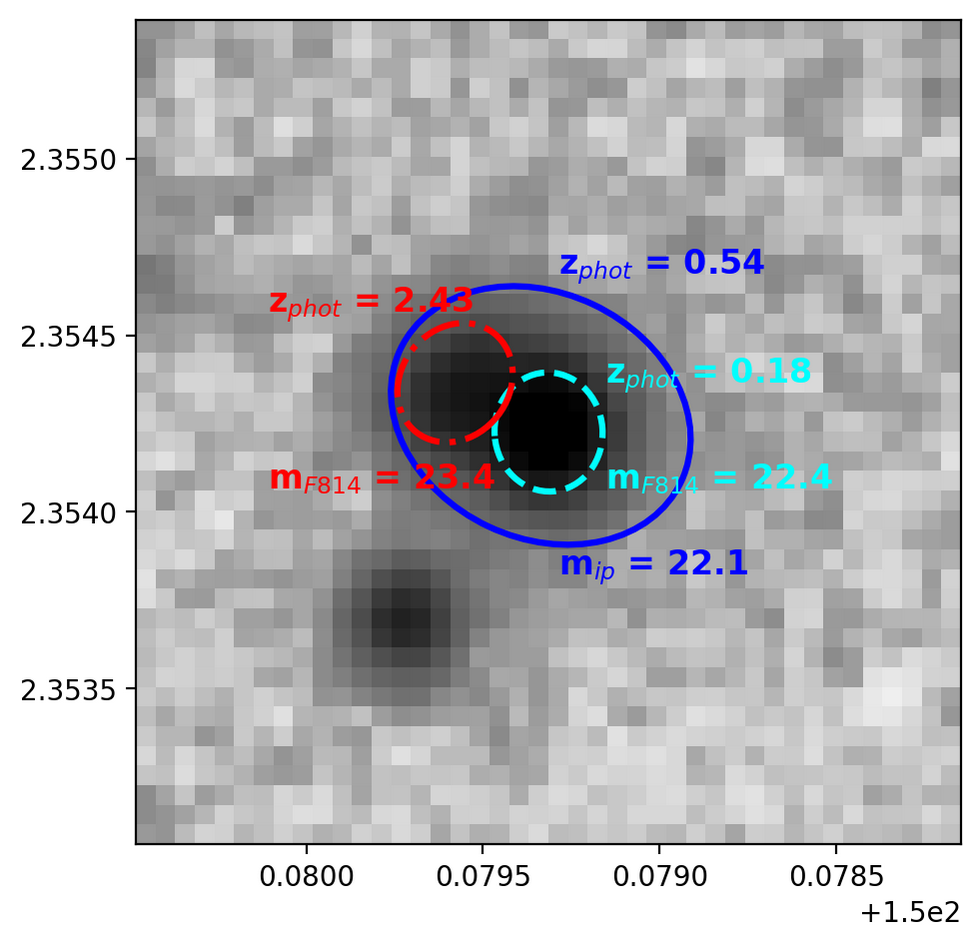
\includegraphics[width=0.33\linewidth]{figs/annotated_blends_lowres2.png}\hfill
	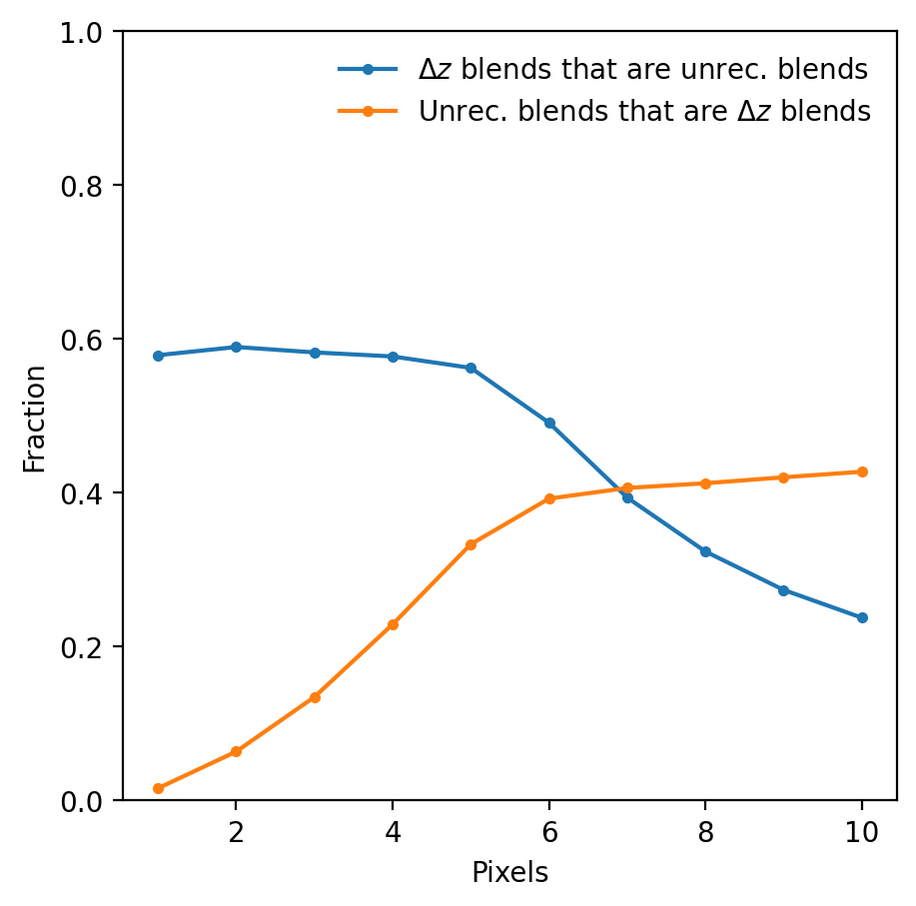
\includegraphics[width=0.33\linewidth]{figs/deltaz_plot}\hfill
	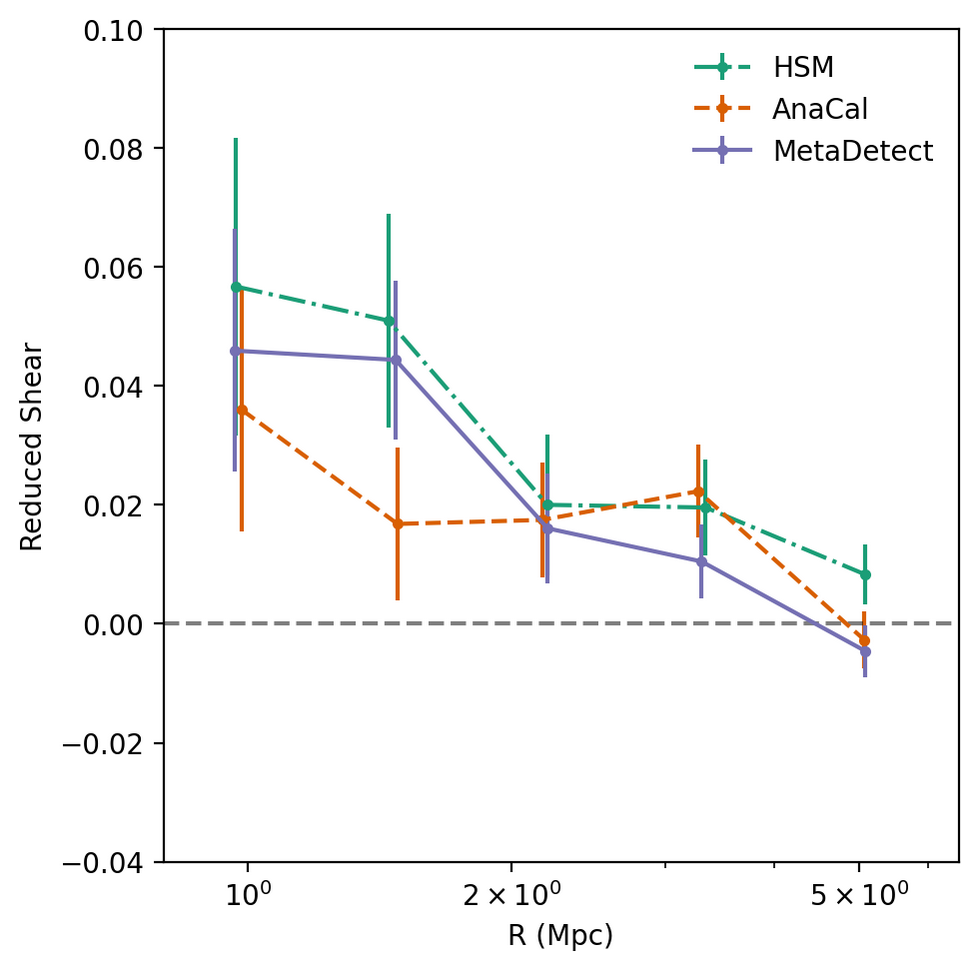
\includegraphics[width=0.33\linewidth]{figs/shear_profiles.png}
	\caption{\textbf{Left:} Example unrecognized blend in COSMOS field. Subaru detection is shown in dark blue with  HST detection in cyan and red. Note that both the photo-$z$ and shape of the Subaru galaxy are a non-linear combination of the HST galaxies. \textbf{Middle:} Fraction of blends with high redshift difference that are labelled as unrecognized blends (in blue) and vice-versa in orange as a function of pixel distance in definition of $\Delta z$ blend. Removing these objects may reduce shear calibration bias. \textbf{Right:} Tangential shear profiles around Abell 360 using three shear calibration schemes, \texttt{Anacal},  \texttt{Metadetect}, and \texttt{shapeHSM}.}
	\label{fig:plot}
\end{figure}

\textbf{Galaxy Clusters:} As part of the Rubin commissioning, I have been working on producing \ul{the first Rubin weak lensing results} by studying the Abell 360 cluster.
% This early science played a pivotal role in stress testing many of the science pipelines along with verification and validation of the telescope's ability to perform weak lensing measurements.
This early science allows us to stress test the science pipelines along with verification and validation of the telescope's ability to perform weak lensing measurements.
% This early science stress tests many of the science pipelines along with verification and validation of the telescope's ability to perform weak lensing measurements.
I primarily focused on source selection to isolate a lensing sample, estimating the $n(z)$ for that lensing sample, and estimating a tangential shear profile using \texttt{Anacal} and \texttt{shapeHSM}.
A preliminary comparison of the profiles using the estimators is shown in the right panel of Fig.~\ref{fig:plot}.
I also created a cross-matched catalog with DESI spectra creating an independent validation set for the photo-z's \cite{dp1_pz}.
Through these experiences, I’ve grown comfortable with the Rubin science ecosystem and would like to use that to continue exploring clusters. 

\indent \indent \textbf{Clusters + unrec. blend:} A natural extension to my cluster work and blending work would be to investigate how the removal of unrecognized blends can improve cluster shear profiles, subsequent mass estimates, and cosmology.
The authors of \cite{manon} have started this study by designing a blending metric for cluster cosmology that was validated in simulation, and I have worked to implement this metric on observational data.
We will test if there are improvements to shear profiles around clusters and their mass estimates by removing the most blended objects.

\indent \indent \textbf{Clusters + Beyond $\Lambda$CDM:} Outside of cluster cosmology, I am interested in studying clusters for their ability to constrain dark matter and test general relativity.
Individual clusters can help constrain self-interacting dark matter and test general relativity through probing the anisotropic stress ($\eta$), while studying the ensemble of clusters can help constrain cosmological parameters like $f\sigma_8(z)$ and $\gamma$ \cite{cluster_gr, erosita}.
I am excited to perform these studies with incoming Rubin Data Preview 2 and Data Release 1 along with any JWST/Euclid/DESI/ROMAN data made public during this time. 
% While there are some previous works \cite{cluster_gr, erosita} on these parameters, there are still exciting prospects to perform these studies with Rubin along with incoming JWST/Euclid/DESI/ROMAN data.
% Given my previous experience with the Rubin ecosystem, along with the timing of Data Preview 2 and Data Release 1 being publicized during the postdoc, I am in prime position to conduct those studies.
% I am excited to perform these studies with Rubin along with incoming JWST/Euclid/DESI/ROMAN data.
\\

% While this is quite different from my previous experiences, I have been successful in producing meaningful results in my diverse interests in the past.

% I developed an improvement to radio telescope array redundant calibration [cite], ran 2D numerical simulations of charges around a boosted black hole finding fractal-like patterns in the basin boundary of the charges [cite], characterized backgrounds in a direct detection search for dark matter using SKIPPER CCDs [cite], and looked for parity violating signatures in Lyman-$\alpha$ data and showed that a naive covariance estimate could produce a large spurious signal [cite].


I have been focusing on unrecognized blend as they are an unavoidable systematic for weak lensing.
Continuing to work on understanding the biases introduced by unrecognized blends in all aspects of galaxy cosmology is vital work that must be done for any ground based galaxy survey like LSST.
While challenging, I am excited to continue working on and learning about unrecognized blends along with studying galaxy clusters to study the universe and probe beyond $\Lambda$CDM cosmology. 


\begin{multicols}{2}
\setstretch{0.8}
\setlength\bibitemsep{0pt}
\printbibliography
\end{multicols}


\end{document}
